\label{sec:Erwartungswerte}

Aus den in Versuchsteil 1 und 2 gemessenen Werten soll nun für den ersten Schritt der Auswertung der theoretisch erreichbare Farbraum berechnet werden. Hierfür werden zuerst die drei farbigen Lichtstrahlen mithilfe des Spektrums der Quecksilberdampflampe und den Transmissionsspektren der dichrotitischen Spiegel berechnet. Aus diesen werden dann die Positionen in der Farbtafel bestimmt, mit welchen der darstellbare Farbraum bestimmt werden kann.

Unter Annahme keiner Verluste an den dichroitischen Spiegeln können mithilfe der in Abschnitt \ref{V1_AUSW} berecheten Transmissionsspektren und des in Abschnitt \ref{V2_AUSW} berechneten Quecksilberdampflampenspektrums die Spektren der Farbstrahlen wie folgt berechnet werden:
\begin{eqnarray}
\Phi_{e\lambda,1}(\lambda) = & \Phi_{e\lambda}(\lambda)\cdot  T_{\lambda,1}(\lambda) \\
\Phi_{e\lambda,2}(\lambda) = & \Phi_{e\lambda}(\lambda)\cdot  T_{\lambda,2}(\lambda) \\
\Phi_{e\lambda,3}(\lambda) = & \Phi_{e\lambda}(\lambda) \cdot T_{\lambda,3}(\lambda)
\end{eqnarray}
Und es ergeben sich für die Strahlen die folgenden drei Spektren:

\begin{figure}[h]
	\centering
	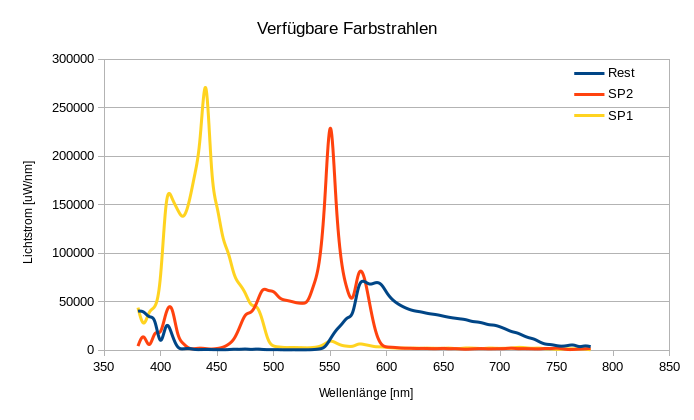
\includegraphics[scale=0.7]{Images/A_Farbstrahlen.png}
	\caption{Spektren der im Beamer aufgespalteten Farbstrahlen (Rot, Grün und Blau)}
\end{figure}
Für jede dieser Farbstrahlen wird nun die Farbkoordinate in der CIE-Normtafel berechnet. Hierfür wird, ausgehend von [\cite[Seite 26]{AML_SKRIPT}], das Spektrum jeder Farbe mit den drei Tristimuluskurven integriert. Die Tristimuluskurven in $5nm$-Schritten werden von [\cite[Seite 34]{AML_SKRIPT}] entnommen. Die Ergebnisse werden nun mit der Summe aller drei Ergebnisse normiert, und es ergeben sich die Koordinaten $x_n$ und $y_n$ wie folgt:

\begin{eqnarray*}
X_n = & \int\limits_{\mbox{380nm}}^{\mbox{780nm}} \Phi_{e\lambda,n}(\lambda)\cdot \overline{x}(\lambda)d\lambda \\
Y_n = & \int\limits_{\mbox{380nm}}^{\mbox{780nm}} \Phi_{e\lambda,n}(\lambda)\cdot \overline{y}(\lambda)d\lambda \\
Z_n = & \int\limits_{\mbox{380nm}}^{\mbox{780nm}} \Phi_{e\lambda,n}(\lambda)\cdot \overline{z}(\lambda)d\lambda \\
x_n = & \frac{X_n}{X_n+Y_n+Z_n} \\
y_n = & \frac{Y_n}{X_n+Y_n+Z_n}
\end{eqnarray*}
Da hier diskrete Werte in 5nm-Schritten für sowohl die Tristimuluskurven als auch die Lichtströme der Farbstrahlen vor liegen, kann hier nicht von Hand integriert werden. Stattdessen wird vereinfacht die Summe der wellenlängenspezifischen Multiplikation der Tristimuluskurve und Lichtstromes verwendet. Durch die hohe Anzahl der Schritte (N=80) ergibt sich ein relativ kleiner Fehler im Vergleich zu einer polynomialen Approximation. Da nach dem Ergebnis der Integrationen normiert wird, ist auch das $d\lambda$ vernachlässigbar. Es wird verwendet:
\begin{equation}
X_n = \sum_{i=0}^{80} \Phi_{e\lambda,n}(i*5nm + 380nm) \cdot \overline{x}(i*5nm + 380nm)
\label{A_SUM}
\end{equation}
Gleichung \ref{A_SUM} wird hier analog für $Y_n$ und $Z_n$ verwendet. In Tabelle \ref{A_COORDS} sind die berechneten Farbkoordinaten aufgelistet.

\begin{table}[h]
\caption{Berechnete erwartete Farbkoordinaten}
\centering
\begin{tabular}{| c | c | c | c | c | c |}
\hline
Strahl (n) & $X_n$ & $Y_n$ & $Z_n$ & $x_n$ & $y_n$ \\
\hline
Blau (1) & 585007 & 160445 & 2756357 & 0.1671 & 0.04582 \\
Grün (2) & 690939 & 1351575 & 316961 & 0.2928 & 0.57283 \\
Rot (3) & 803518 & 595402 & 26823 & 0.5636 & 0.4176 \\
\hline
\end{tabular}

\label{A_COORDS}
\end{table}
Der daraus resultierende theoretisch abbildbare Farbraum ist in Abschnitt \ref{A_FCOORDS}, Abbildung \ref{A_Farbdreieck} dargestellt. Er überschneidet sich zu 68\% mit dem sRGB-Farbraum, bzw. zu 49\% mit dem Adobe-RGB-Farbraum. Da das betrachtete Farbdreieck vollständig in den beiden Farbräumen liegt, wird diese Übereinstimmung durch Berechnung des relativen Flächeninhaltes kalkuliert. Dies ist für den betrachteten Beamer durchaus zu erwarten, da dieser aus Kostengründen mit hoher Wahrscheinlichkeit keine möglichst genaue Farbwiedergabe besitzten wird. Blau- und Grüntöne sind erwartungsgemäß weit außen, der Rotton jedoch ist relativ schwach ausgeprägt. Betrachtet man das Spektrum der Quecksilberdampflampe, so ist zu erkennen, dass die Lichtquelle selbst schon im Bereich des roten Lichtes weitaus weniger intensiv strahlt als in den grünen und blauen Wellenlängen.